\documentclass{beamer}\usetheme{boxes}

\usepackage{amsmath,hyperref}

\newcommand{\Mp}{\ensuremath{{M_{+}}}}
\newcommand{\barMp}{\ensuremath{\overline{\Mp}}}
\newcommand{\Dt}{\ensuremath{\Delta t}}
\newcommand{\tM}[1]{\ensuremath{\tilde{M}(#1)}}
\newcommand{\tMt}{\tM{\tau}}
\newcommand{\tMB}{\ensuremath{{\tilde{M}_B}}}
\newcommand{\tE}[1]{\ensuremath{{\tilde{E}(#1)}}}
\newcommand{\tEt}{\tE{\tau}}

\newcommand{\bskip}{\\~\\}
\usepackage{Sweave}
\begin{document}
\input{sunbelt13-pres-concordance}
\title{Detection of Small Covert Networks Embedded in Large Networks}
\author{Carl~A.~B.~Pearson \inst{1} \and Burton H. Singer \inst{1} \and Edo Airoldi \inst{2}}
\institute{\inst{1}Emerging Pathogens Institute, University of Florida \and \inst{2}Harvard University
}
\frame{\titlepage}

\frame{
\frametitle{TODO FUNDING INFORMATION}
}

\frame{
\frametitle{Overview}
\begin{itemize}
\item Definitions,
\item A Model to Reflect Those,
\item Implementation for a Particular Case: Salafi Jihadi Network,
\item Detecting Groups in this Model,
\item Some Detection Results for that Implementation, and
\item Flaws, Extensions, and Outlook
\end{itemize}
}

\frame{
\begin{block}{What is {\em Covert}?}
{\em a covert network} is a sub graph where interaction information is some combination of unavailable, unreliable, or (mostly) indistinguishable from the enclosing graph structure
\end{block}
\begin{block}{\ldots or Operationally}
A relatively small, organized group of conspirators, masking their existence via communication discipline and taking advantage of a noisy background.

For this particular talk: Salafi Jihadi network.

Note: not that group's more recent focus on {\em leaderless jihad}.
\end{block}
}

\usebackgroundtemplate{
\vbox to \paperheight{\vfil\hbox to \paperwidth{\hfil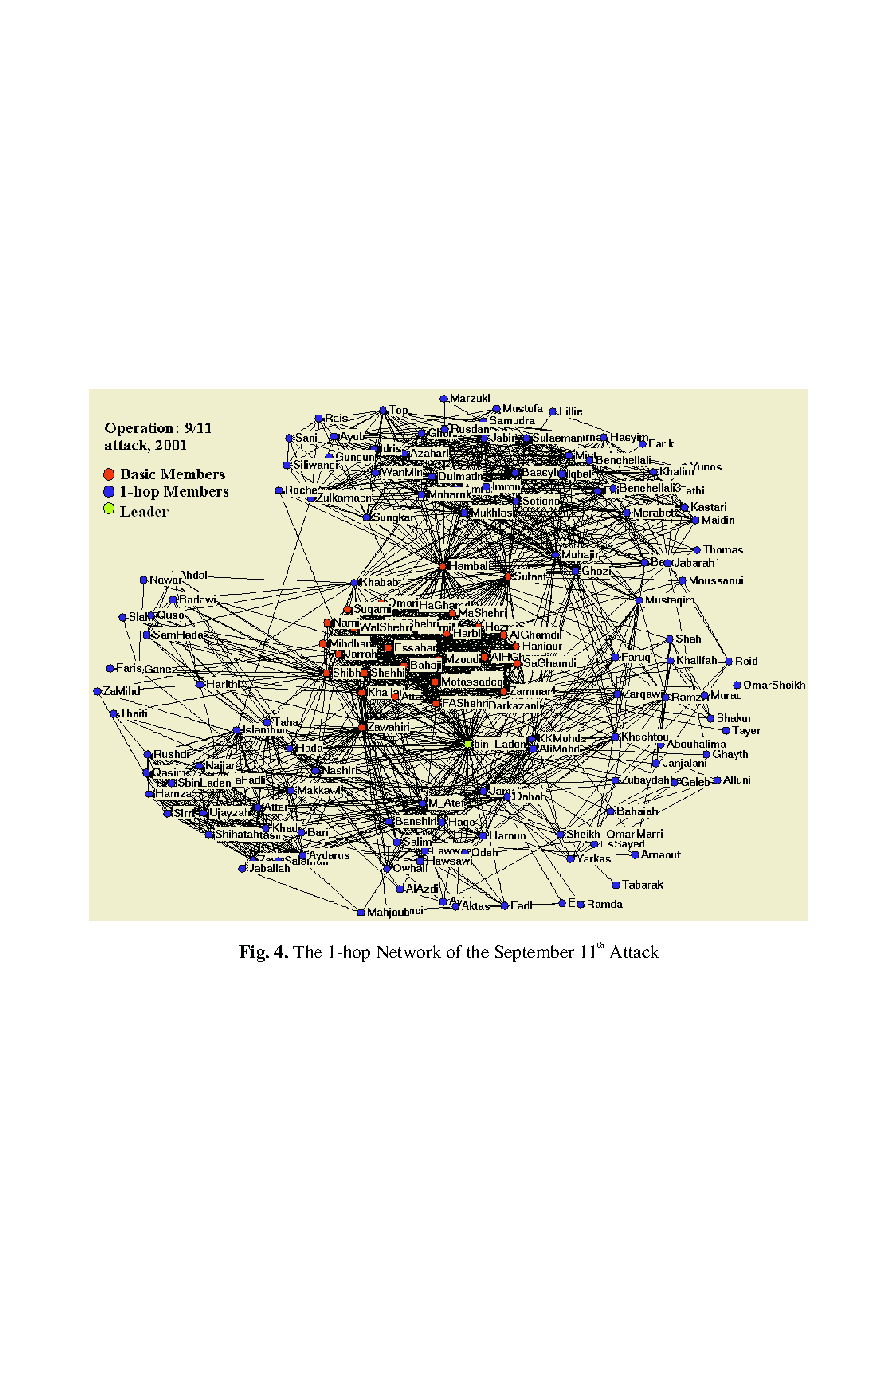
\includegraphics[width=0.9\paperheight,height=0.9\paperheight]{sageman_crop.pdf}\hfil}\vfil} }
\frame{
}
\usebackgroundtemplate{}

\frame{
\frametitle{A General Model}
\begin{block}{Salient Features}
\begin{itemize}
\item isolated, but highly interconnected subordinate groups, and
\item bridging middle managers,
\item with some tradecraft,
\item ``lost'' among myriad public communications
\end{itemize}
\end{block}
}

\frame{
\frametitle{Our Implementation addressing Salafi Jihadi Network}
For our simple model of a bomber group in Salafi Jihadi Network
\begin{description}
\item[population] many small cliques, which are recursively cliqued into single graph
\item[covert leader] stochastically added to cliques, outgoing connections to a random member of each of the covert groups
\item[subordinates] few, medium size cliques with connections between clusters
\item[communications] simple message content {\em Good} vs. {\em Bad}
\end{description}
}

\frame{
\frametitle{\ldots or Symbolically}
\begin{itemize}
\item a structured population, $P$,
\item covert leader(s), $H$,
\item subordinate covert group(s), $\{C_i\}$,
\item stochastic behavior model for intra- and inter-group messages
\end{itemize}
}

\frame{
\frametitle{Aside: Sales Pitch}
Scala-based Implementation available for review/remix:
\bskip
\href{https://github.com/pearsonca/scala-commsim}{https://github.com/pearsonca/scala-commsim}
\bskip
Actively moving from closed, non-Scala implementation to that repository.  Please request changes, point out bugs, etc.
\bskip
Also, this presentation:
\bskip
\href{https://github.com/pearsonca/sunbelt13-presentation}{https://github.com/pearsonca/sunbelt13-presentation}
}

\usebackgroundtemplate{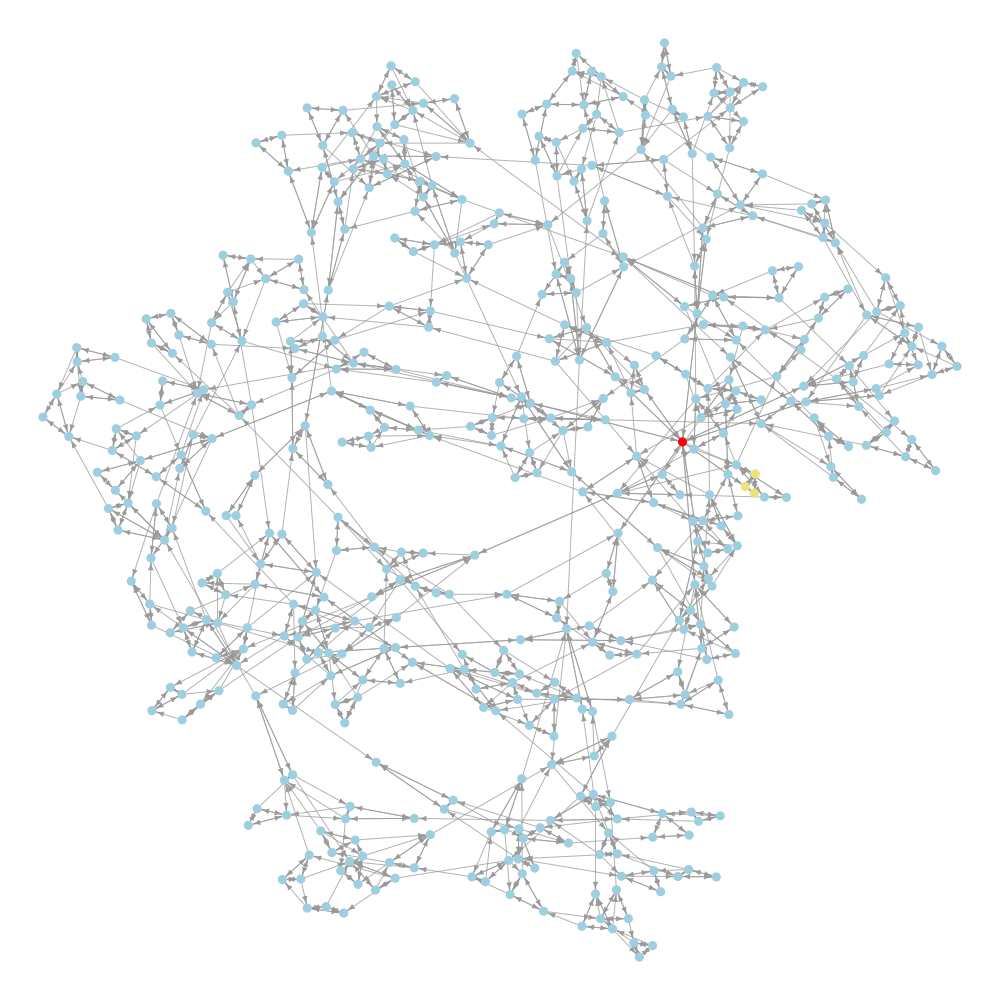
\includegraphics[width=0.9\paperheight,height=0.9\paperheight]{3_1_500.png}}
\frame{
\begin{columns}[t]
\begin{column}{0.7\textwidth}\end{column}
\begin{column}{0.3\textwidth}
3 clique, 1\%\ remix
\end{column}
\end{columns}
}
\usebackgroundtemplate{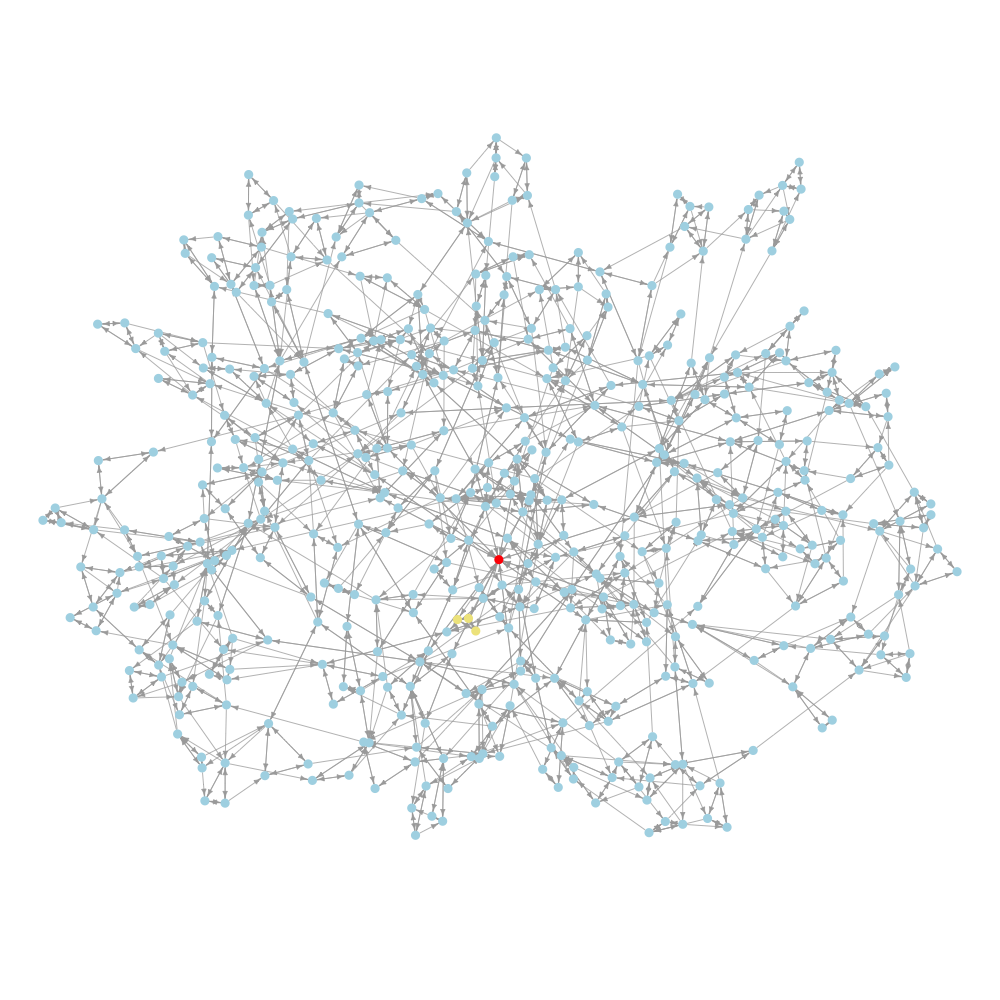
\includegraphics[width=0.9\paperheight,height=0.9\paperheight]{3_10_500.png}}
\frame{
\begin{columns}[t]
\begin{column}{0.7\textwidth}\end{column}
\begin{column}{0.3\textwidth}
3 clique, 10\%\ remix
\end{column}
\end{columns}
}
\usebackgroundtemplate{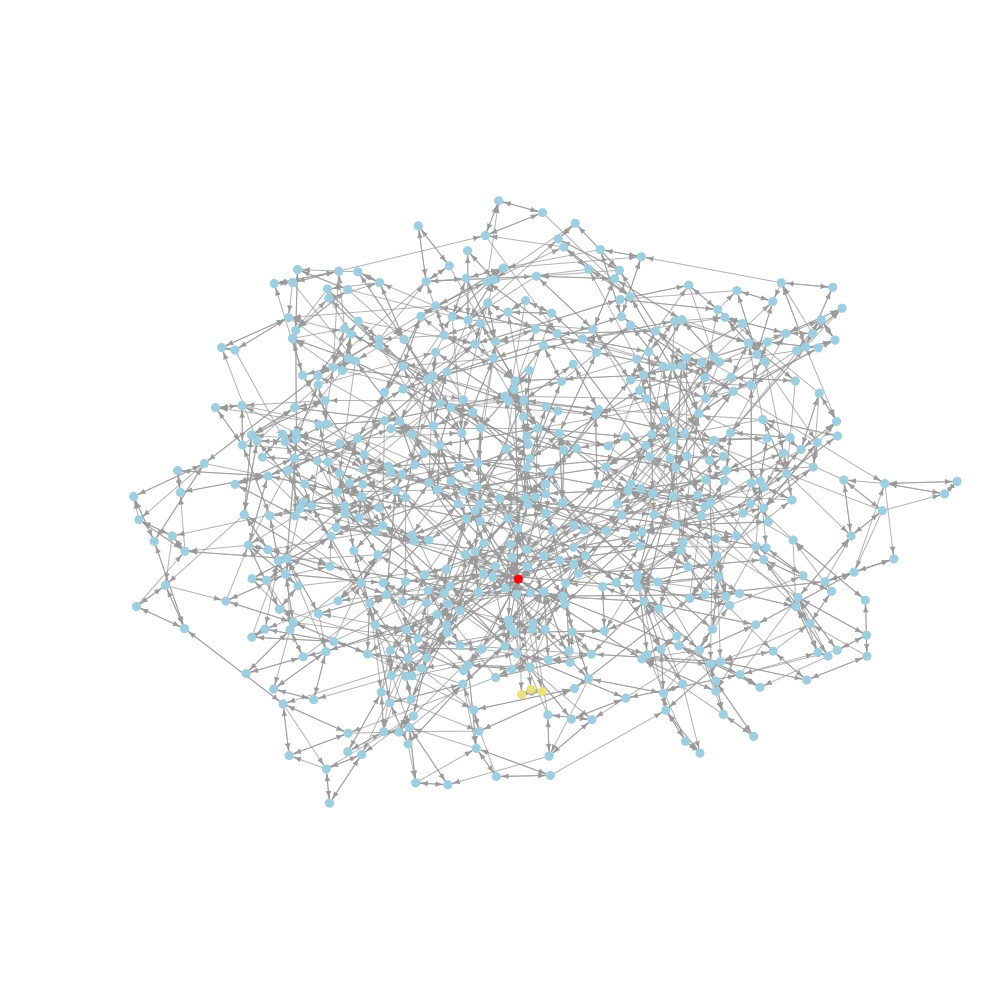
\includegraphics[width=0.9\paperheight,height=0.9\paperheight]{3_30_500.png}}
\frame{
\begin{columns}[t]
\begin{column}{0.7\textwidth}\end{column}
\begin{column}{0.3\textwidth}
3 clique, 30\%\ remix
\end{column}
\end{columns}
}
\usebackgroundtemplate{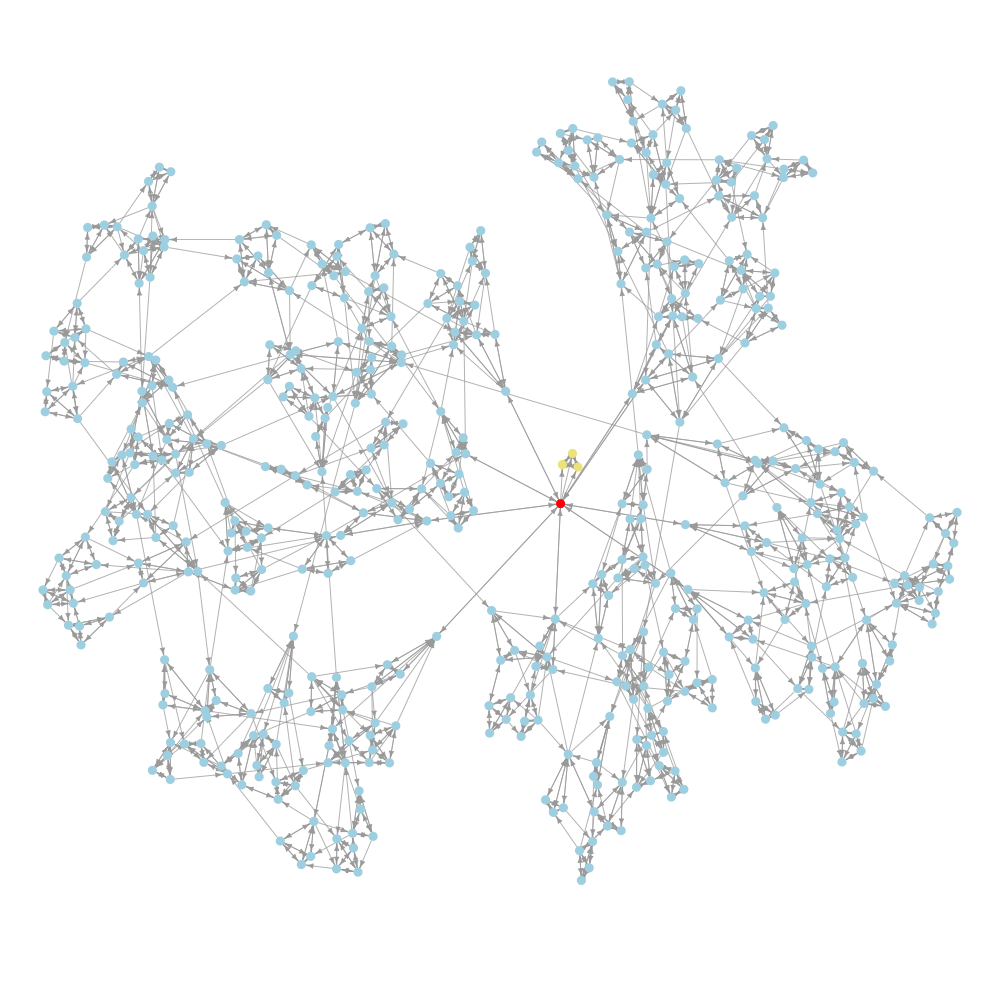
\includegraphics[width=0.9\paperheight,height=0.9\paperheight]{4_1_500.png}}
\frame{
\begin{columns}[t]
\begin{column}{0.7\textwidth}\end{column}
\begin{column}{0.3\textwidth}
4 clique, 1\%\ remix
\end{column}
\end{columns}
}
\usebackgroundtemplate{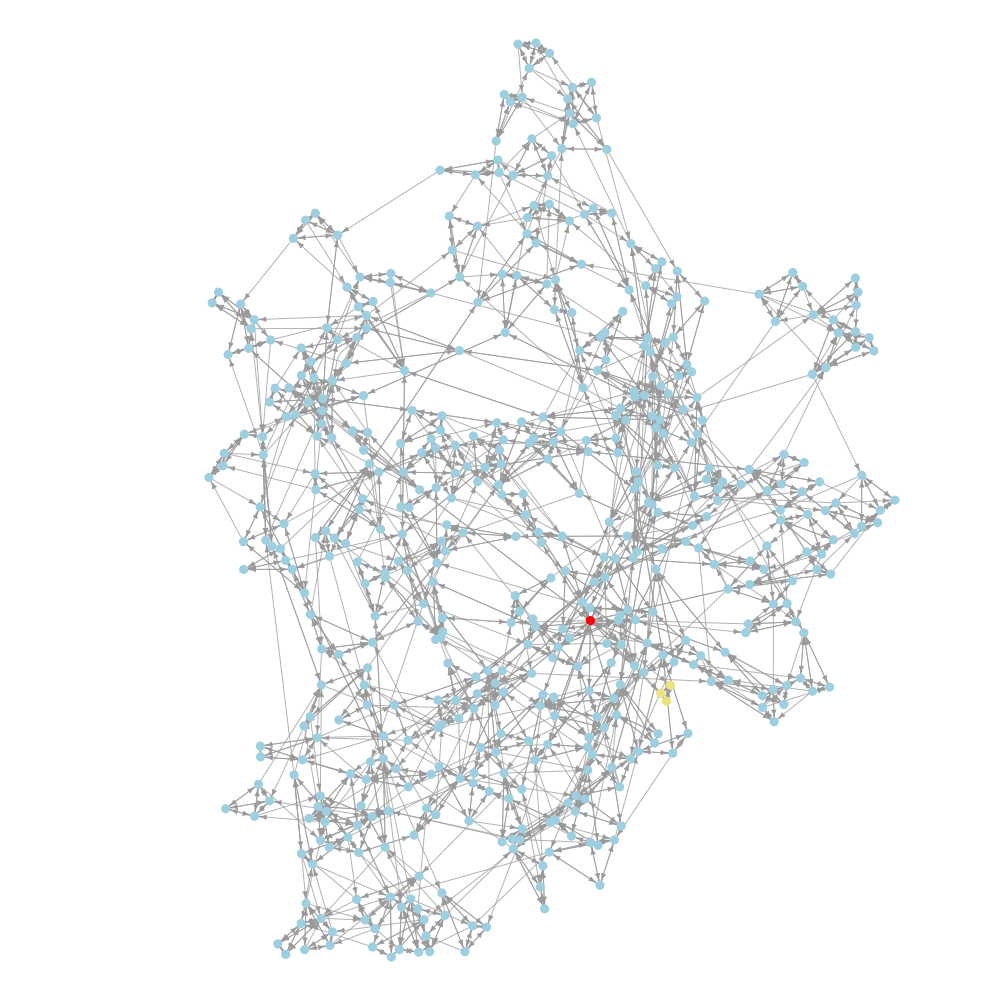
\includegraphics[width=0.9\paperheight,height=0.9\paperheight]{4_10_500.png}}
\frame{
\begin{columns}[t]
\begin{column}{0.7\textwidth}\end{column}
\begin{column}{0.3\textwidth}
4 clique, 10\%\ remix
\end{column}
\end{columns}
}
\usebackgroundtemplate{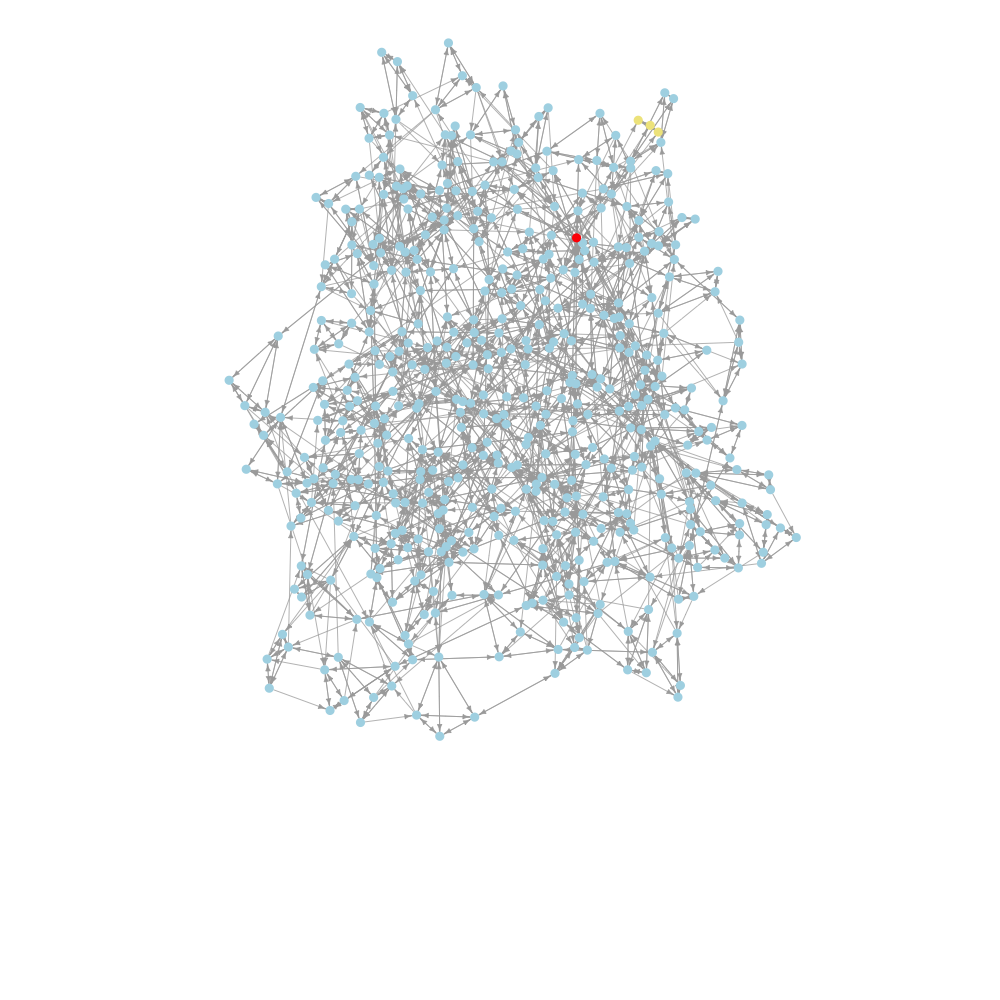
\includegraphics[width=0.9\paperheight,height=0.9\paperheight]{4_30_500.png}}
\frame{
\begin{columns}[t]
\begin{column}{0.7\textwidth}\end{column}
\begin{column}{0.3\textwidth}
4 clique, 30\%\ remix
\end{column}
\end{columns}
}
\usebackgroundtemplate{}


\frame{
\frametitle{Real Time Challenges to Detection}
\begin{itemize}
\item population vs. covert group communication network initially unknown,
\item potentially limited resources for monitoring those communications,
\item thus gathered information unreliable / incomplete,
\item and risk trade-offs: FPR \&\ TPR vs. action by group
\end{itemize}
% notes-notes-notes
}

\frame{
\frametitle{Our Model: The Observer}
An algorithmic description of
\begin{itemize}
\item the data limitations (e.g., random suppression or transformation of signals), and
\item detection strategy(ies)
\end{itemize}
}

\frame{
\frametitle{Some Simple Strategies}
\begin{itemize}
\item pure content: pick up everyone that has sent and received a {\em Bad} message
\item pure structural: pick up highest degree person and all people below median
\item mixed structural and content
\end{itemize}
}

\frame{
\frametitle{Appropriate Measures?}
Assume that any given plot has some critical amount of planning-related communication.

But what else?
\begin{itemize}
\item true positive rate,
\item false positive rate,
\item resource investment
\end{itemize}

% not obvious how to transform planning-related communication rate, so use a post for the other TPR, FPR
}


\frame{
\frametitle{Results For These Modes}
TODO series of plots
}

\frame{
\frametitle{Flaws, Extensions, and Outlook}
\begin{itemize}
\item limited vocabulary -- add message diversity, require content detection as well,
\item unsophisticated Observer model and strategies -- add resource model, shifting strategies
\item background / foreground structural generations -- new generators, fitting to live traffic
\end{itemize}
}

% \frame{
% \frametitle{INSERTING AN R-GENERATED FIGURE}
% \begin{figure}
% \begin{center}
%<<plotfig1,fig=TRUE,echo=FALSE>>=
% # periodT <- 366; omega <- 2*pi/periodT
% # monthDays<-c(31,29,31,30,31,30,31,31,30,31,30,31)
% # monthOffset<- -(rev(cumsum(monthDays)) + -periodT/2)
% # monthInset<- monthOffset + 15
% # fun <- function(x) { cos(omega*x) }
% # cplot <- function() {
% # plot(fun, xlim=c(-periodT/2,periodT/2), 
% #      xlab="",yaxt="n",xaxt="n",ylab="Mosquito Abundance",type="l",col="blue")
% # axis(side=1, at=c(monthOffset,periodT/2), labels=F)
% # axis(side=1, at=monthInset, labels=c("JAN","FEB","MAR","APR","MAY","JUN","JUL","AUG","SEP","OCT","NOV","DEC"),tick=F, cex.axis=0.7)
% # }
% # cplot()
%@
% \end{center}
% \end{figure}
% % notes-notes-notes
% }

% \frame{
% \frametitle{INSERT ANOTHER PDF}
% \begin{figure}
% \begin{center}
% \includegraphics[width=0.9\textwidth]{insert.pdf}
% \caption{Bicout et al. J. Med. Entomol. 43(5): 936-946 (2006)}
% \end{center}
% \end{figure}
% % this is a not uncommon measurement of a seasonally varying vector population.
% }

% \usebackgroundtemplate{\includegraphics[width=0.9\paperheight,height=0.9\paperheight]{template-plotfig1.pdf}}
% \frame{
% \frametitle{USE PREVIOUSLY GENERATING THING AS BACKGROUND}
% \begin{itemize}
% \item with
% \item some
% \item text
% \item over it
% \end{itemize}
% }
% \usebackgroundtemplate{}


% \frame{
% \frametitle{SEVERAL EQUATIONS}
% \begin{align*}
% E(t) &= \begin{cases}
%         \dfrac{\Mp}{\Dt} & t \in \Dt \\
%         0 & \textrm{otherwise}
%         \end{cases}\tag{Step} \\
% E(\rho, t) &= \begin{cases}
%         \dfrac{2\Mp}{\Dt(2-\rho)} & t \in \Dt(1-\rho) \\
%         \dfrac{2\Mp}{\Dt(2-\rho)\rho}\left(1-\dfrac{2|t|}{\Dt}\right) & t \in \rho\Dt \\
%         0 & \textrm{otherwise}
%         \end{cases}\tag{Modified Step} \\
% E(t) &= \dfrac{2\Mp}{\Dt}\sqrt{\dfrac{2}{\pi}}e^{-\dfrac{8t^2}{\Dt^2}}\tag{Approximate $\delta$}
% \end{align*}
% }

% \frame{
% \frametitle{USING COLUMNS EXAMPLE}
% \begin{columns}[t]
% \begin{column}{0.3\textwidth}
% TEXT LEFT, FIG RIGHT
% \end{column}
% \begin{column}{0.7\textwidth}
% \begin{figure}
% \begin{center}
% \includegraphics[width=1.1\textwidth]{justone.pdf}
% \end{center}
% \end{figure}
% \end{column}
% 
% \end{columns}
% % notes-notes-notes
% }

\end{document}
